\documentclass[a4paper,11pt]{article}
\usepackage{graphicx}
\usepackage[left=1cm, right=2cm, top=2cm, bottom = 1.5cm]{geometry}

\begin{document}
	\begin{flushleft}
	 	\begin{Huge}
			\textbf{Yadnyi V. Deshpande}
		\end{Huge}
	\end{flushleft}

	%\begin{flushleft}
		\begin{minipage}[b]{0.4\textwidth}
			\raggedright
			5/416 DRP Road,\par
			Near Vyankatrao Highschool,\par
			Padma Power Laundry, \par
			Ichalkaranaji,\par
			Maharashtra, India.
		\end{minipage}%
		\begin{minipage}[b]{0.3\textwidth}
			\raggedright
			\begin{large}
				(+91)7741033079\par
				\centering
				\raggedright
				deshpandeyadnyi@gmail.com\par
				\centering  
				\raggedright
				https://github.com/yadnyi\par
			\end{large}
		\end{minipage}%
		\begin{minipage}[b]{0.3\textwidth}
			\centering
			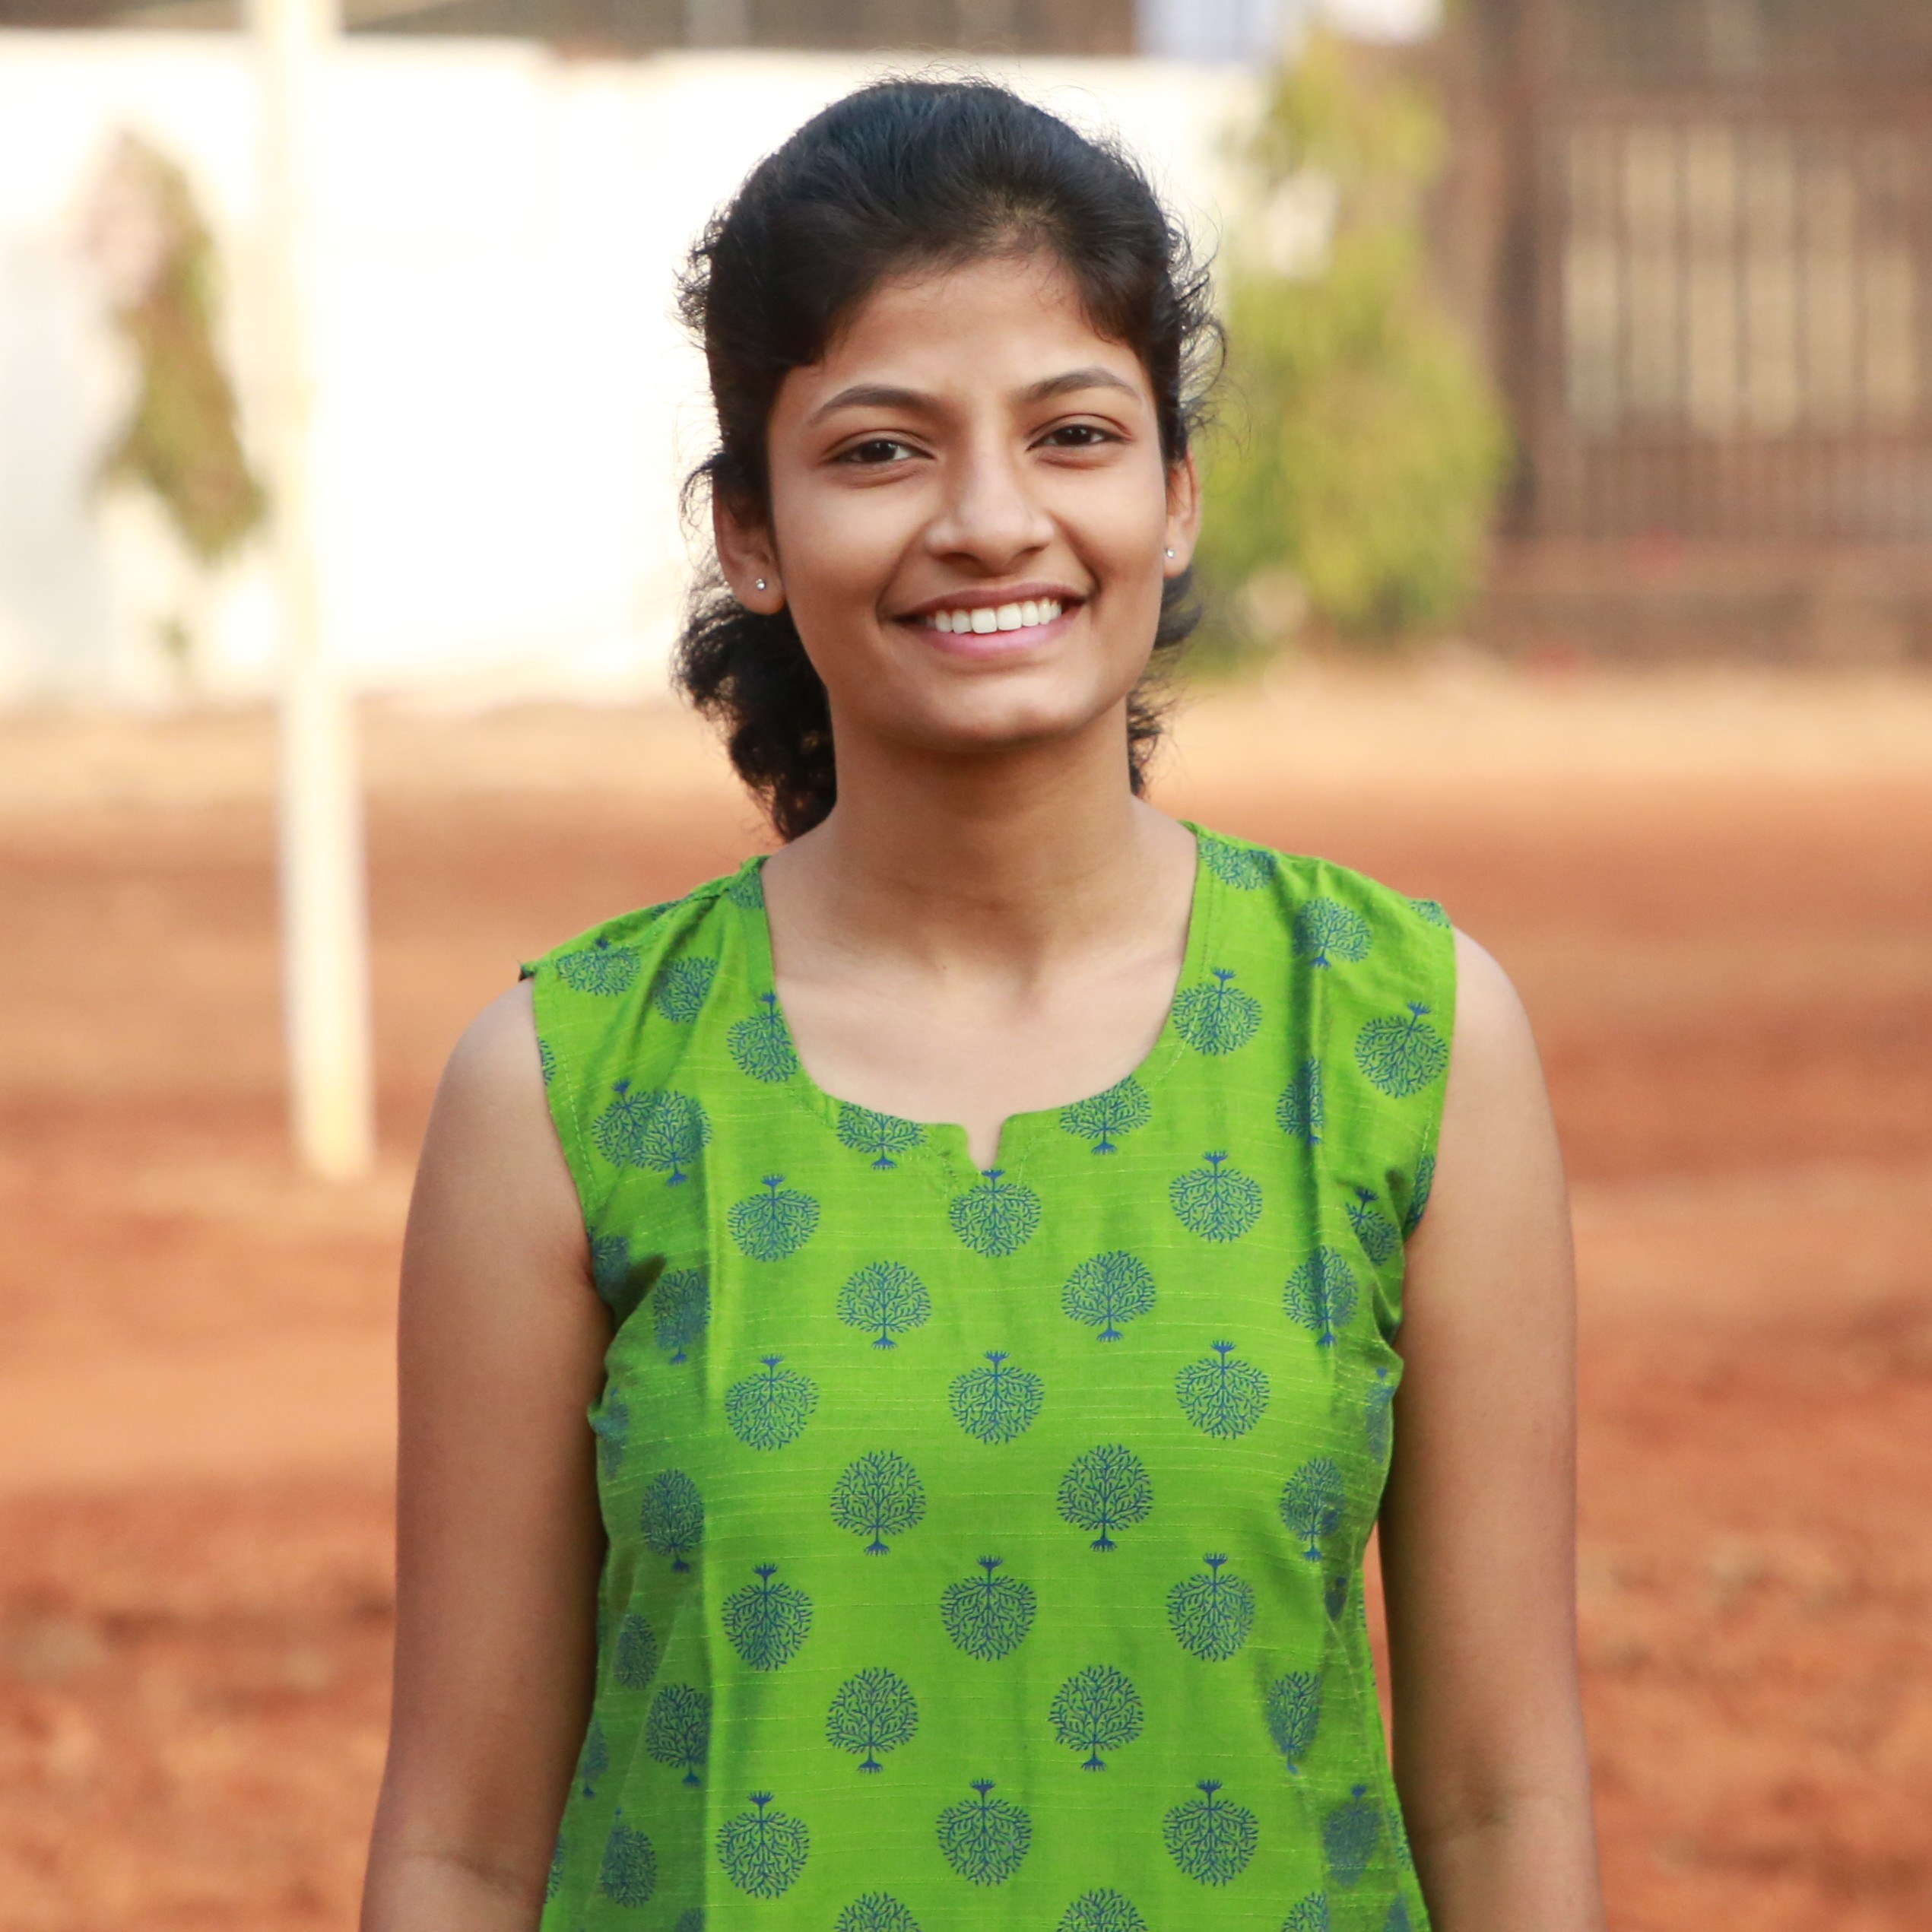
\includegraphics[width = 30mm, height = 30mm]{yadnyi.JPG}
		\end{minipage}%
		
\noindent\rule{18.59cm}{0.4pt}	

\begin{minipage}[t]{1\textwidth}
			\raggedright\smallskip
			\begin{Large}
				\textbf{Career objective:}\medskip\linebreak%
				{\small To be a part of internship program where I can learn under professionals to gain knowledge and improvement to my skills as well as contribute to the organization along the way.}\linebreak%
			\end{Large}
		\end{minipage}%
		\vspace{0.35cm}

\begin{Large}
	\textbf{Projects:}\medskip\linebreak%
\end{Large}

\begin{minipage}[b]{0.5\textwidth}
	\begin{itemize}
			\raggedright
			\item {\textbf{Thirsty Crow:}
				\begin{itemize}
				  	\item {\footnotesize Bot traverses arena using line follower and pick-drop the magnetic objects.
				  	\item \underline {Technology Stack}: Embedded C programming, Python, Blender, OpenGL}
				\end{itemize}}

			\item {\textbf{Huffman code for Compression and Decompression:}
						\begin{itemize}
						  	\item {\footnotesize Compresses and decompresses the text file.
						  	\item \underline {Technology Stack}: C language(Stack, Queue etc.)}
				        \end{itemize}}
	\end{itemize}			         
\end{minipage}%				
\begin{minipage}[b]{0.5\textwidth}
	\begin{itemize}
			\raggedright

			\item {\textbf{Hostel Allotment Portal:} 
						\begin{itemize}
						  	\item {\footnotesize Domains of allotment like login page, allotment process etc.
						  	\item \underline {Technology Stack}: HTML-CSS, JAVASCRIPT for frontend and MYSQL, PHP, database for backend. }
				        \end{itemize}}

				    \item {\textbf{Music Player:} 
						\begin{itemize}
						  	\item {\footnotesize All basic features of music player.
						  	\item \underline {Technology Stack}: Python, Tkinter library for GUI, Pygame- Mixer for sound playing}
				        \end{itemize}}


	\end{itemize}
				        
\end{minipage}% 

\begin{minipage}[t]{0.5\textwidth}
			\raggedright\smallskip
			\begin{LARGE}
				\Large \textbf{Extra Curricular Activities:}\medskip%
				{\small
					\begin{itemize}
						\item {\textbf{Campus Management Co-ordinator} at Technical Event Of COEP - MINDSPARK'18.}
						\item {\textbf{Event Co-ordinator} at Cultural Event of COEP - IMPRESSIONS'18.}
						\item {\textbf{Vocalist} at COEP Cultural (Music) team.}
						\item {\textbf{SPIC MACAY} [Nationwide - The Society for the Promotions of Indian Classical Music and Culture Amongst Youth] Volunteer }
					\end{itemize}
				}
			\end{LARGE}
			\vspace{0.5cm}
\begin{LARGE}
			\textbf{Co-curricular Activities:}\medskip%
				{\small
					\begin{itemize}
						\item {Part of \textbf{Katalyst} Program for women Engineers.}
						\item {Member of \textbf{Computer Society Of India(CSI)}- Pune Chapter}.
					\end{itemize}
				}
				
			\end{LARGE}
			\vspace{0.5cm}
\begin{LARGE}
				\Large \textbf{Technical Skills:}\medskip%
				{\small
					\begin{itemize}
						\item {C, Python.}
						\item {HTML-CSS, PHP, JAVASCRIPT,MYSQL.}
						\item {Web Development, DBMS}
					\end{itemize}
				}
			\end{LARGE}
			
			\vspace{0.7cm}
\end{minipage}%
\hspace{0.6cm}
\begin{minipage}[t]{0.5\textwidth}
			\raggedright\smallskip
			\begin{LARGE}
				\textbf{Achievements:}\medskip%
				{\small
					\begin{enumerate}
						\item \textbf{1st Runner-up} in \textbf{eYantra National Robotics Competition 2018}
						\item \textbf{Finalist}in Mindspark'18 \textbf{Hackathon 3.0} .
						\item \textbf{Distinction in Visharad Pratham}, in Indian Classical Singing by Akhil Bhartiy Gandharv Mahavidyalay(2015).
						\item \textbf{2nd Runner-up}in State level singigng Competition MIC-DROP at BMCC, Pune.
						\item \textbf{1st rank} in SSC Kolhaput Board with \textbf{98.80\%}.
						%\item \textbf{State level 16th rank} in MTS exam in 9th standard.\linebreak
					\end{enumerate}
				}
			\end{LARGE}
			\vspace{0.65cm}

\begin{Large}
				\textbf{Training:}\medskip%
				{\small
					\begin{itemize}
						\item {Python Workshop conducted by CSI.}
						\item {Katalyst Training for self awareness, self concepts and values, etc.}
						\item {Katalyst Training for Basics of C Programming}.
					\end{itemize}
				}
			\end{Large}

			\
\end{minipage}%

\begin{Large}
	\textbf{Education:}\medskip%
\end{Large}

 \begin{large}
			\bigbreak
			%\textbf{Education}
			\begin{tabular}{|c |c |c |c |c |}
				\hline
				Degree & College / School  & Passing Year & Pass Percentage \\
				\hline
				B.Tech(SY IT)& College of Engineering, Pune& 2021 & 7.48\\
				\hline
				HSC &Vyankatrao Jr. College, Ichalkaranji & 2017 & 89.85\% \\
				\hline
				SSC & Ichalkaranji High School, Ichalkaranji & 2015 & 98.80 \%\\
				\hline
				 
			\end{tabular}
\end{large}
\vspace{0.5cm}

\begin{minipage}[t]{0.4\textwidth}
			\raggedright\smallskip
			\begin{LARGE}
				 \textbf{Soft Skills:}\medskip%
				{\small
					\begin{itemize}
						\item {Communication Skills.}
						\item {Leadership.}
						\item {Time Management.}
						\item {Team Player.}
					\end{itemize}
				}
				
			\end{LARGE}
			\vspace{0.5cm}	

\end{minipage}%
\hspace{0.6cm}

\end{document}

